\subsection{Lệnh primes}
\underline{\textbf{Chức năng của lệnh:}} Lệnh \verb|primes| in ra các số nguyên tố từ 2 đến 280 qua phương pháp sàng Eratosthenes \cite{mit-xv6} \cite{primes}.

\textbf{Phương pháp sàng Eratosthenes:}
\begin{enumerate}[labelindent=1em, labelsep=0.2cm, leftmargin=1cm, wide=\parindent, topsep=0.1cm, itemsep=-1ex, partopsep=1.5ex, parsep=1.5ex]
	\item Lập danh sách các số tự nhiên từ 2 đến $n$.
	\item Đánh dấu số đầu tiên (đặt là $a$) chưa bị gạch bỏ trong danh sách là số nguyên tố.
	\item Loại bỏ các số là bội của $a$. Lặp lại từ bước 2 cho đến khi không còn đánh dấu được số nào nữa.
\end{enumerate}

\begin{figure}[htp!]
	\centering
	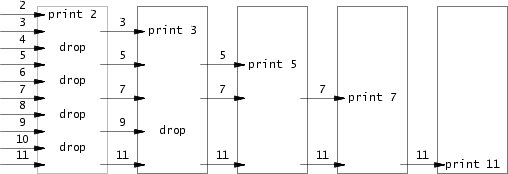
\includegraphics[width=0.9\textwidth]{figures/Eratosthenes-sieve}
	\caption{Hình minh họa thuật toán sàng Eratosthenes}
\end{figure}

\underline{\textbf{Thiết lập thuật toán:}}

Hàm \mintinline{C++}|void primes(int pL)|:
\begin{enumerate}[labelindent=1em, labelsep=0.2cm, leftmargin=1cm, wide=\parindent, topsep=0.1cm, itemsep=-1ex, partopsep=1.5ex, parsep=1.5ex]
	\item Đọc số đầu tiên trong đường dẫn \verb|pL| (\verb|pL| là một đường dẫn đã được thiết lập trước, chứa các số chưa được đánh dấu/chưa bị loại bỏ khỏi danh sách). Nếu không đọc được số nào thì kết thúc hàm, ngược lại thì in số đó ra màn hình.
	\item Thiết lập một đường dẫn (pipe) dùng để lưu các số chưa được đánh dấu/chưa bị loại bỏ khỏi danh sách.
	\item Phân chia tiến trình ra làm hai. Tiến trình cha xử lý việc loại bỏ các số là bội của số đầu tiên, trong khi tiến trình con thì gọi đệ quy hàm \verb|primes|.
\end{enumerate}

Lệnh sẽ báo lỗi khi người dùng nhập sai cú pháp.

\underline{\textbf{Khó khăn đã gặp phải:}}
\begin{itemize}[labelindent=1em, labelsep=0.2cm, leftmargin=1cm, wide=\parindent, topsep=0.1cm, itemsep=-1ex, partopsep=1.5ex, parsep=1.5ex]
	\item Hiểu và xử lí được cách dãy số được truyền qua lại giữa các tiến trình.
	\item Vì tài nguyên của xv6 có hạn, nên các mô tả tệp sẽ phải đóng ngay và được đóng một cách hợp lí để tránh ảnh hưởng tới quá trình xử lí.
\end{itemize}

Dưới đây là kết quả kiểm tra lệnh \verb|primes| bằng chương trình kiểm thử:
\begin{figure}[htp!]
	\centering
	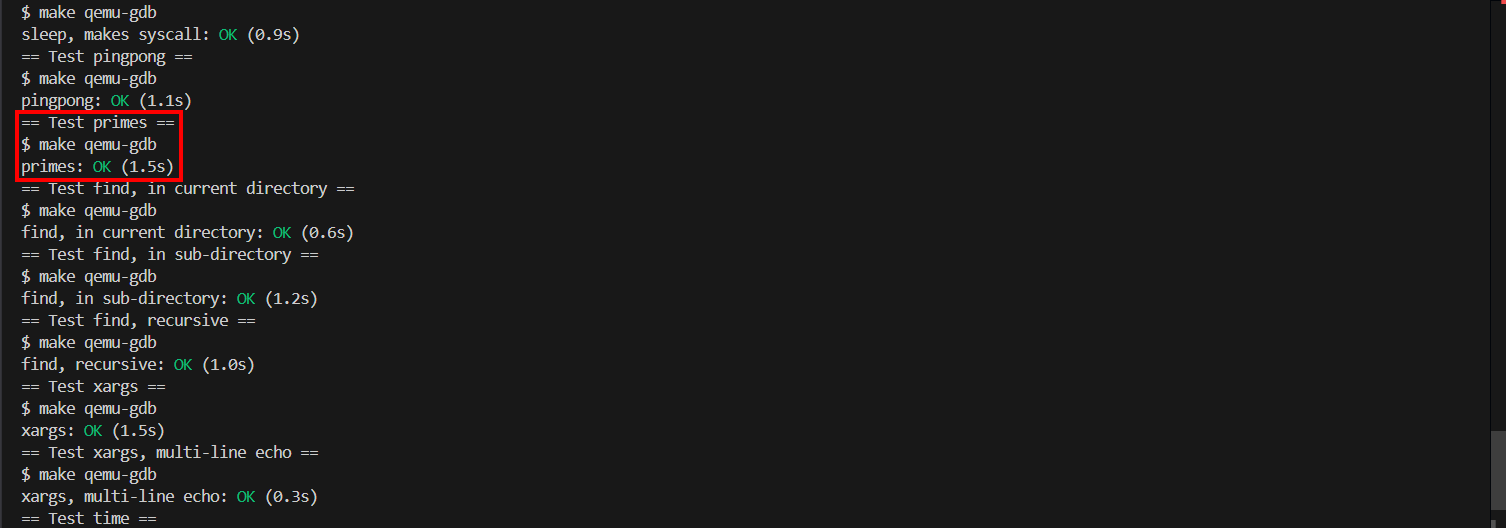
\includegraphics[width=0.9\textwidth]{figures/primes-test}
	\caption{Kết quả kiểm thử \textbf{primes} bằng công cụ chấm bài \textbf{grade} của MIT}
\end{figure}